%%% template.tex
%%%
%%% This LaTeX source document can be used as the basis for your technical
%%% paper or abstract. Intentionally stripped of annotation, the parameters
%%% and commands should be adjusted for your particular paper - title, 
%%% author, article DOI, etc.
%%% The accompanying ``template.annotated.tex'' provides copious annotation
%%% for the commands and parameters found in the source document. (The code
%%% is identical in ``template.tex'' and ``template.annotated.tex.'')

\documentclass[conference]{acmsiggraph}

\TOGonlineid{45678}
\TOGvolume{0}
\TOGnumber{0}
\TOGarticleDOI{1111111.2222222}
\TOGprojectURL{}
\TOGvideoURL{}
\TOGdataURL{}
\TOGcodeURL{}

\title{Rendering Metaballs with PBRT}

\author{Vinícius Vendramini\thanks{e-mail:todo@email.com}\\IME-USP \and Wilson K. Mizutani\thanks{e-mail:kazuo@ime.usp.br}\\IME-USP}
\pdfauthor{Vinícius Vendramini, Wilson K. Mizutani}

\keywords{implicit surface, metaball, mesh generation, ray tracing}

\begin{document}

%% \teaser{
%%   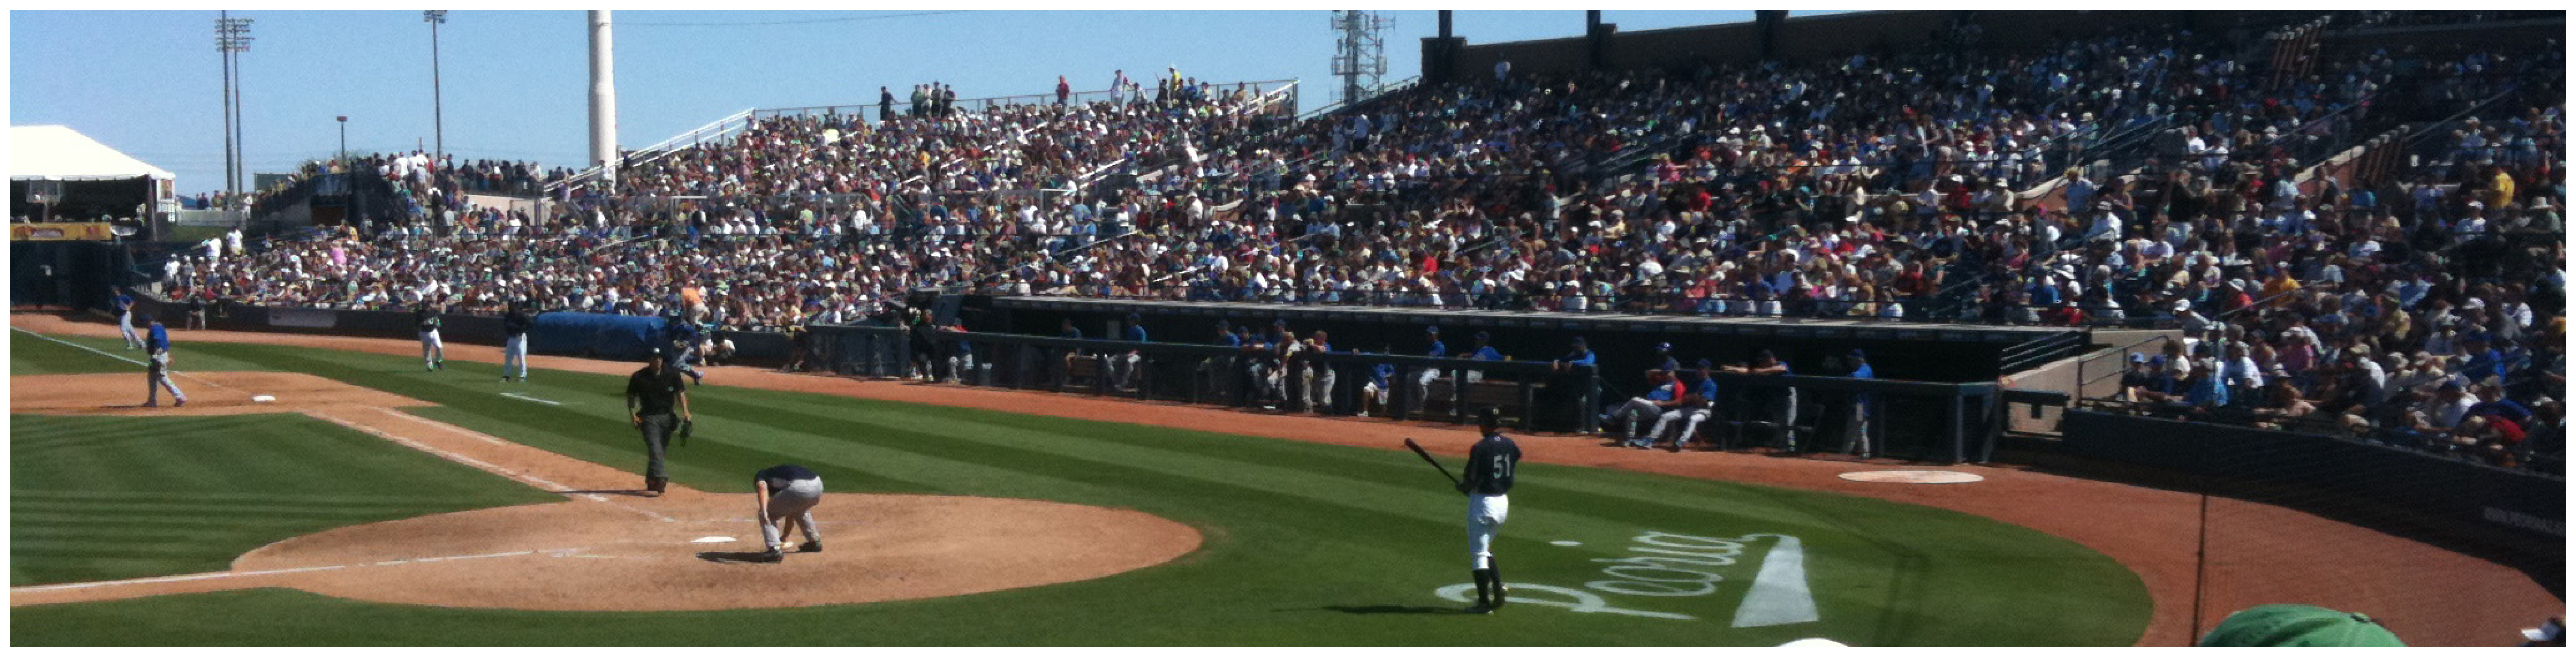
\includegraphics[height=1.5in]{images/sampleteaser}
%%   \caption{Spring Training 2009, Peoria, AZ.}
%% }

\maketitle

\begin{abstract}

Citations can be done this way~\cite{Jobs95} or this more concise 
way~\shortcite{Jobs95}, depending upon the application.

\end{abstract}

%\begin{CRcatlist}
%  \CRcat{I.3.3}{Computer Graphics}{Rendering Metaballs with PBRT}{Implicit surfaces}
%  \CRcat{I.3.7}{Computer Graphics}{Rendering Metaballs with PBRT}{Ray-tracing};
%\end{CRcatlist}

\keywordlist

%% Use this only if you're preparing a technical paper to be published in the 
%% ACM 'Transactions on Graphics' journal.

\TOGlinkslist

%% Required for all content. 

\copyrightspace

\section{Introduction}

\subsection{PBRT}

\subsection{Metaballs}

\subsection{Approaches}

\section{Marching cubes algorithm}

%% Explicar algoritmo

\subsection{Ambiguous cases}

\begin{equation}
 \sum_{j=1}^{z} j = \frac{z(z+1)}{2}
\end{equation}

\begin{eqnarray}
x & \ll & y_{1} + \cdots + y_{n} \\
  & \leq & z
\end{eqnarray}

\section{Analytic intersection}


\begin{figure}[ht]
  \centering
  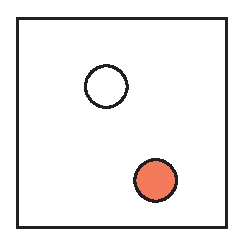
\includegraphics[width=1.5in]{images/samplefigure}
  \caption{Sample illustration.}
\end{figure}

\section{Implmentation}

\subsection{Marching cubes}

\subsection{Intersection}

\section{Conclusion}

Lorem ipsum dolor sit amet, consectetur adipisicing elit, sed do
eiusmod tempor incididunt ut labore et dolore magna aliqua. Ut enim ad
minim veniam, quis nostrud exercitation ullamco laboris nisi ut
aliquip ex ea commodo consequat. Duis aute irure dolor in
reprehenderit in voluptate velit esse cillum dolore eu fugiat nulla
pariatur. Excepteur sint occaecat cupidatat non proident, sunt in
culpa qui officia deserunt mollit anim id est laborum.

\subsection{Future works}

\section*{Acknowledgements}

%TODO

\bibliographystyle{acmsiggraph}
\bibliography{template}
\end{document}
